% Klassifiziert den Dokumenten-Typ
% Doku: http://exp1.fkp.physik.tu-darmstadt.de/tuddesign/
% Farben: http://www.tu-darmstadt.de/media/medien_stabsstelle_km/services/medien_cd/das_bild_der_tu_darmstadt.pdf
%  bigchapter: Chapter haben doppelte Schriftgröße
%  linedtoc: Linien im Inhaltsverzeichnis wie bei Überschriften
%  colorbacktitle: Der Dokumenten-Titel wird mir der Accentfarbe hinterlegt
\documentclass[bigchapter,colorback,accentcolor=tud4b,linedtoc,11pt]{tudreport}

% Input Dokument hat das Encoding UTF-8
\usepackage[utf8]{inputenc}
% Wichtiges Paket für Links und verlinktes Inhaltsverzeichnis
\usepackage[ngerman]{hyperref}
% Paket für Fußnoten
\usepackage[stable]{footmisc}
% Paket für Bibliotheks-Verzeichnis, square: Verwende eckige statt runde klammern
% \usepackage[square]{natbib}
% Paket zum Plotten von Datensätzen
\usepackage{pgfplots}
% Verwende deutsche Bezeichner für Inhaltsverzeichnis, ... (ngerman = New German: neue Rechtschreibung)
\usepackage{ngerman}
% Modul für chemische Formeln
\usepackage{chemformula}
% Deutsche Zahlen (entfernt z.B. das Leerzeichen nach einem Dezimal-Komma)
\usepackage{ziffer} 

\usepackage[verbose]{placeins}

%\usepackage{graphicx}
%\usepackage{caption}
\usepackage{subcaption} %Für subfigures

% PDF-Optionen
\hypersetup{
  pdftitle={TU Darmstadt \- Physikalisches Praktikum für Fortgeschrittene},
  pdfauthor={Manuel Kress und Sören Link},
  pdfsubject={Versuch 4.9},
  pdfview=FitH,
}
% Nummeriere formeln in Subsections einzeln
\numberwithin{equation}{subsection}
% Kleines makro zur assymetrischen Fehlerangabe
\def\tol#1#2#3{\hbox{\rule{0pt}{15pt}${#1}^{+{#2}}_{-{#3}}$}}% 

% Entspricht-Zeichen
\usepackage{scalerel}

\newcommand\equalhat{%
\let\savearraystretch\arraystretch
\renewcommand\arraystretch{0.3}
\begin{array}{c}
\stretchto{
    \scalerel*[\widthof{=}]{\wedge}
    {\rule{1ex}{3ex}}%
}{0.5ex}\\ 
=%
\end{array}
\let\arraystretch\savearraystretch
}
%BEGINN TITELSEITE

\title{Laserresonator}

\subtitle{Manuel Kress  \\Sören Link}

\subsubtitle{Betreuer: Patric Ackermann \hfill Versuchsdatum: 10. Februar 2014}

\author{Manuel Kress, Sören Link}

\settitlepicture{img/title.jpg}

\institution{Physikalisches Praktikum \\für Fortgeschrittene \\ Versuch 4.9}

\date{\today}


%ENDE TITELSEITE

\begin{document}
%ANFANG DOKUMENT

%Titelseite einfügen
\maketitle

%Inhaltsverzeichnis einfügen
\tableofcontents

%ANFANG INHALT

\chapter{Einleitung}

\chapter{Grundlagen}
\section{Laserprinzip}
Die Grundvorraussetzung für jeden Laser ist die Besetzungsinversion. Dazu müssen sich für zwei Energieniveaus im Lasermedium, zwischen denen ein Übergang durch Emission von Photonen erlaubt ist, im energetischeren Niveau mehr Atome befinden als im weniger energetischen. Nur wenn diese Voraussetzung erfüllt ist, können spontan emmitierte Photonen mehr Emission als Absorption anregen, da beide vorgänge proportional zur Anzahl der Atome in den zugehörigen Energieniveaus sind.

Da die Einsteinkoeffizienten für stimulierte Emission und Absorption gleich groß sind ($B_{12}=B_{21}$), ist es unmöglich, ein 2-Niveau System zum lasern anzuregen, da unabhängig von der Stärke des Pumpvorgangs und unter Vernachlässigung der spontanten Emission maximal gleichbesetzung der Niveaus 1 und 2 erreicht werden kann.

Aus diesem Grund benutzt man für Laser zumeist 3- oder 4-Niveau Systeme. Dabei werden durch den Pumpvorgang Atome vom Grundniveau $E_0$ auf ein kurzlebiges niveau $E_1$ angeregt. Dieses geht sehr schnell durch spontane Emission in den langlebigen Zustand $E_{L1}$ über. 3- und 4-Niveau Systeme unterscheiden sich dadurch, dass im 3-Niveau System der Laservorgang von $E_{L1}$ nach $E_{0}$ stattfindet, wärend im 4-Niveau System ein kurzlebiger Zustand $E_{L2}$ zwischengeschaltet ist. Dies erlaubt das Betreiben von Lasern mit einem 4-Niveau System bei bereits sehr geringer Pumpleistung, da auch bei sehr geringer Anregung bereits Besetzungsinversion zwischen den relevanten Laser-Niveaus besteht.

Beim HeNe-Laser im speziellen werden Helium-Atome durch Gasentladungen von einem Grundzustand in die Zustände $2^{9}S_{1}$ und $2^{0}S_{0}$, welche beide metastabil sind, angeregt. Die so angeregten Heliumatome geben ihre Energie durch stöße an das Neon ab, welches dadurch in den 3s bzw 2s Zustand angeregt wird. Ermöglicht wird dieser Energietransfer durch den Geringen Energieunterschied der betroffenen Helium- und Neon Energieniveaus. Der Laserforgang selbst erfolg dann beim Übergang der Neon-Atome von dem 3s zum 2p Zustand, letzterer geht dann relativ schnell durch spontane Emission in den 1s Zustand über, welcher nach Stößen mit der Wand des Verstärkermediums in den Grundzustand übergeht.

\begin{figure}[ht!]
\centering
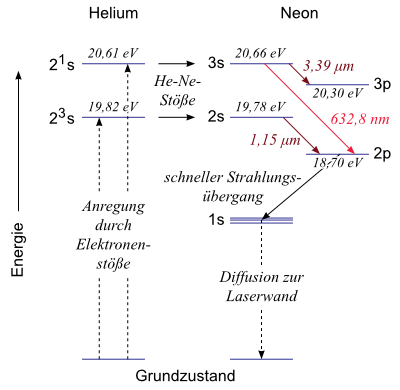
\includegraphics[width=65mm]{img/5074.png}
\caption{Energieschema eines HeNe-Lasers}
\label{HeNeLaser}
\cite{HeNeNiveaus}
\end{figure}
\section{Laserozillatoren}
Ein optischer Oszillator ist ein optischer Aufbau innerhalb dessen Licht hin- und her oszillieren kann. Im einfachsten Sinne besteht ein optischer Oszillator aus zwei in einem Abstand \(L\) gegenüberstehenden, planparallelen Spiegeln. Innerhalb dieser beiden Spiegeln wird Licht immer wieder von der einen Seite zur anderen reflektiert. Es schwingen also innerhalb des Oszillators stehende Lichtwellen. Da aber an den Orten der Spiegel die Wellenfunktionen jeweils verschwinden müssen, können sich nur stehende Wellen ausbilden, welche einen Knoten an den Spiegelpositionen haben. Für die Wellenlängen dieser stehenden Wellen gilt \(\lambda_n = \frac{2L}{n}\). Alle Lichtwellen anderer Wellenlängen werden durch destruktive Interferenz ausgelöscht. Für die Wellenlängen \(\lambda_n\) ist der Oszillator also ein Resonator.

Bei einem Laser wird das Lasermedium in eines solchen Resonator gebracht. Jedesmal wenn eine Lichtwelle durch den Laserresonator und damit durch das Lasermedium läuft, wird diese durch das Laserprinzip (siehe oben) verstärkt. Verstärkt werden aber nur jene Lichtwellen mit einer Wellenlänge von \(\lambda_n\). Die durch den Resonator verstärkten Frequenzen \(\nu_n = \frac{c}{\lambda_n}\) haben also einen Frequenzabstand \(\Delta\nu\) von

$$ \Delta\nu = \frac{c}{2L} $$

wobei $c$ die Lichtgeschwindigkeit im Vakuum ist. \(\Delta\nu\) nennt sich auch Modenabstand oder freier Spektralbereich des Laserresonators.

\section{Verstärkungsbandbreite}

Natürlich läuft der Laser nicht auf allen Frequenzen $\nu_n$, sondern nur auf jenen, welche überhaupt durch das Lasermedium erzeugt werden. Die Breite des Spektrums des Lasermediums ist durch drei wesentliche Effekte gegeben: Natürliche Linienbreite, Dopplerverbreiterung und Druckverbreiterung.




\section{Resonatortheorie}

\section{Gefahren durch Laserstrahlung}

\chapter{Durchführung}
\section{Ausgangsleistung des Lasers in Abh. von der Resonatorlänge}
Zur Bestimmung der Stabilitätsgrenze des Resonators wurde die Ausgangsleistung für 11 Resonatorlängen aufgenommen, wobei eine Resonatorlänge innerhalb von 2 cm der errechneten Stabilitätsgrenze befand.
Die Spiegel des Laserresonators wurden dazu symmetrisch zum Verstärkermedium voneinander entfernt und die Ausgangsleistung des Resonators wurde mit dem S120C Messkopf, angeschlossen an PM100D Messgerät, aufgenommen. Anschließend wurde versucht, die aufgenommene Leistung durch Justage des Laserrohrs und der Resonatorspiegel zu optimieren.

Zu erwarten war hierbei eine annährend konstante Leistung des Lasers bis einige cm vor der Stabilitätsgrenze, mit einem kleinen Einbruch bei etwa der halben Stabilitätsgrenze.

Als Fehler für die jeweilige Spiegelposition wurden 1.5mm angenommen. Der Fehler für die aufgenommene Leistung wurde über die Fluktuation am Leistungsmessgerät abgeschätzt

\begin{center}
\begin{figure}[h]
\begin{tikzpicture}
\begin{axis}[
    title={Ausgangsleistung des Laserresonators in Abhängigkeit der Resonatorlänge},
    xlabel=Resonatorlänge in cm,
    ylabel=Ausgangsleistung in mW,
    width=0.9\textwidth,
    height= 11cm,
    xmin=20,
    xmax=92,
    grid=both,
    ymin=0,
    ymax=0.6,
    tick align=outside,
    tickpos=left,
    minor x tick num=3,
    minor y tick num=4,
    minor grid style={dotted,thin}
]
\addplot[only marks, mark=x, mark size=3pt, error bars/.cd, y dir=both, x dir=both]
table[x index={0},y index={2}, x error index ={1}, y error index={3}] {messdaten/ausgangsleistung.lvm};
\end{axis}
\end{tikzpicture}
\captionof{figure}{Ausgangsleistung des Laserresonators in Abhängigkeit der Resonatorlänge. Zu sehen ist die annährend konstante Leistugn des Resonators bis hin zu etwa 88cm und der Abfall der Leistung bei etwa der halben Stabilitätsgrenze und bei 89cm Resonatorlänge. Fehlerbalken sind eingezeichnet aber zu klein um sie zu sehen}
\end{figure}
\end{center}

\FloatBarrier
\section{Strahlbreite der Grundmode in Abh. von der Resonatorlänge}
Zur Bestimmung der Strahlbreite \(w\left(\frac{L}{2}\right)\) der Grundmode am Resonatorausgang in Abhängigkeit von der Resonatorlänge \(L\) wurde für 10 verschiedene Resonatorlängen ein Querschnitt durch die $TEM_{00}$ Mode mit einer CCD-Kamera aufgenommen. Um nur die Grundmode anzuregen, wurde das Laserrohr verkippt, bis alle anderen Moden durch Beugungsverluste eliminiert waren.

Hierbei ist zu erwarten, dass die Strahlbreite $w\left(\frac{L}{2}\right)$ mit zunehmender Resonatorlänge \(L\) mit der Beziehung 
$$w\left(\frac{L}{2}\right)=w_0\cdot\sqrt{1+\left({\frac{L}{2 z_0}}\right)^2}$$
zunimmt. Die Strahlbreite \(w\) bei einem Gauß-Stral ist im allgemeinen als die Breite des axialen Profils gegeben, an dem die Intensität des Strahls auf $\frac{1}{e^2}$ der Maximalintensität abgefallen ist. \(z_0=\frac{\pi w_0^2}{\lambda}\) bezeichnet die Rayleigh-Länge mit der Wellenlänge \(\lambda\) des Lichtes und der breite des Strahles \(w_0\) an der Strahltaille. \(z_0\) und damit auch \(w_0\) ist über den Krümmungsradius $R(z)$ der Wellenfront des Gauß-Strahles im Abstand z gegeben:
$$R(z) = z \left(1+\left(\frac{z_0}{z}\right)^2\right)$$
Es gilt nämlich an der Spiegelposition \(z_S\) ist der Radius der Wellenfront \(R(z_S)\) gleich dem Spiegelradius \(r_s\).


\FloatBarrier
\section{Longitudinale Modensruktur in Abh. von der Resonatorlänge}
Die Longitudinale Modenstruktur wurde bestimmt, indem für alle 10 Resonatorlängen die $TEM_{00}$ Mode durch eine Iris und auf auf ein Fabry-Perot Interferometer gelenkt wurde. Das Ausganssignal des Interferometers wurde dann mit einem Digitaloszilloskop verarbeitet.
Da die optische Achse des Laserresonators nicht perfekt kalibiriert war, war bei jeder Messung eine Nachjustierung der Position des Interferometers notwendig. Zwar gelang es uns für jede Resonatorlänge die Longitudinalen Moden mit dem Interferometer aufzunehmen, teilweise erscheinen die Lorenz-Peaks allerdings etwas verwaschen.

Für den Abstand der Longitudinalen Moden im Resonator ist folgender Zusammenhang zu erwarten:
$$\Delta\nu=\frac{c}{2L}$$
\FloatBarrier
\newpage
\section{Verstärkungsbandbreite des HeNe-Lasers}
Zur Bestimmung der Verstärkungsbandbreite des HeNe-Lasers wurde die Länge des Resonators auf 81cm eingestellt. Anschließend wurde das Laserrohr so justiert, dass nur noch die $TEM_{00}$ Mode angeregt wird. Das so angeregte Verstärkungsprofil wurde nun bei einer Ausgangsleistung der Mode von etwa 191mW mit Hilfe eines digitalen Oszilloskops über mehrere Sekunden hinweg aufgenommen. Anschließend wurde das Laserrohr so verkippt, dass auf Grund von Beugungsverlusten die Leistung auf etwa 101mW reduziert abfiel. Im Anschluss wurde erneut das Verstärkungsprofil der $TEM_{00}$ Mode aufgenommen.

\begin{figure}[ht!]
\centering
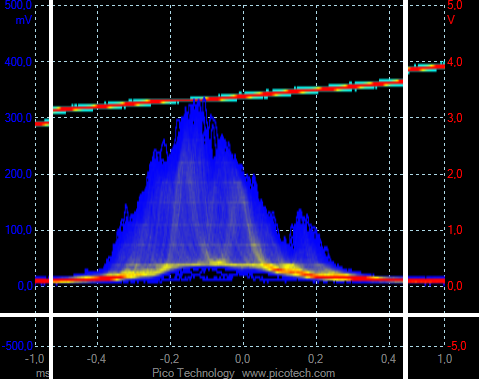
\includegraphics[width=80mm]{Messdaten/81cm191mW4uW.png}
\caption{Verstärkungsprofil des HeNe-Lasers bei einer Ausgangsleistung von etwa 191mW. Für bessere Sichtbarkeit des relevanten bereichs wurden teile der Achsen entfernt. Das Bild ist im Original im Anhang beigefügt}
\label{HeNeBreite191mW}
\end{figure}
\begin{figure}[ht!]
\centering
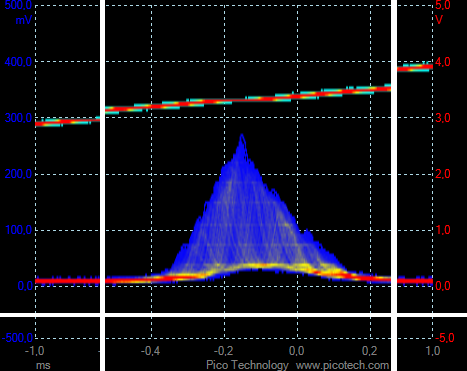
\includegraphics[width=80mm]{Messdaten/81cm101mW4uW.png}
\caption{Verstärkungsprofil des HeNe-Lasers bei einer Ausgangsleistung von etwa 101mW. Für bessere Sichtbarkeit des relevanten bereichs wurden teile der Achsen entfernt. Das Bild ist im Original im Anhang beigefügt}
\label{HeNeBreite101mW}
\end{figure}
\FloatBarrier
Während bei der zweiten Messung wie zu erwarten ein deutlicher Intensitätsabfall zu erkennen ist, scheint die Breite des Verstärkungsprofils annähend gleich zu sein.
\section{Beobachtung höherer transversaler Moden}
Zur Beobachtung höhrer Transversaler Moden wurde ein Drahtkreuz in den Laserresonator eingebracht, um die $TEM_{00}$-Mode zu unterdrücken. Dies erlaubte es, durch gezieltes verkippen des Resonators, höhere Moden anzuregen. Die so angeregten höheren Moden wurden wie in 3.2 mit einer CCD Kamera aufgenommen. Um Rauschen zu unterdrücken wurde dabei über etwa eine Sekunde an Messdaten gemittelt. Da höhere Moden im Gegensatz zut $TEM_{00}$ Mode nicht rotationssymmetrisch sind, mussten die so aufgenommenen Messdaten noch rotiert werden, um einen Modenverlauf symmetrisch zu Paralellen der x- und y-Achsen zu erreichen.

Für die eindimensionale Intensitätsverteilung der Moden ist folgender Zusammenhang zu erwarten
$$I_{n}(x) = I_0 \cdot  H_y \left( \frac{x}{w} \right)^2 \exp \left( \frac{-x^2}{w^2} \right)  $$
\cite{TransModeIntensity}
wobei $H_k$ das k-te Hermitische Polynom ist.

Folgende Daten wurden aufgenommen. Die Diagramme zeigen jeweils die Intensitätsverteilung entlang der in den Bildern gezeigten Schnitte parallel zur x- bzw. y-Achse (oben nach unten, links nach rechts).

\begin{figure}[h]
        \centering
        \begin{subfigure}{0.5\textwidth}
                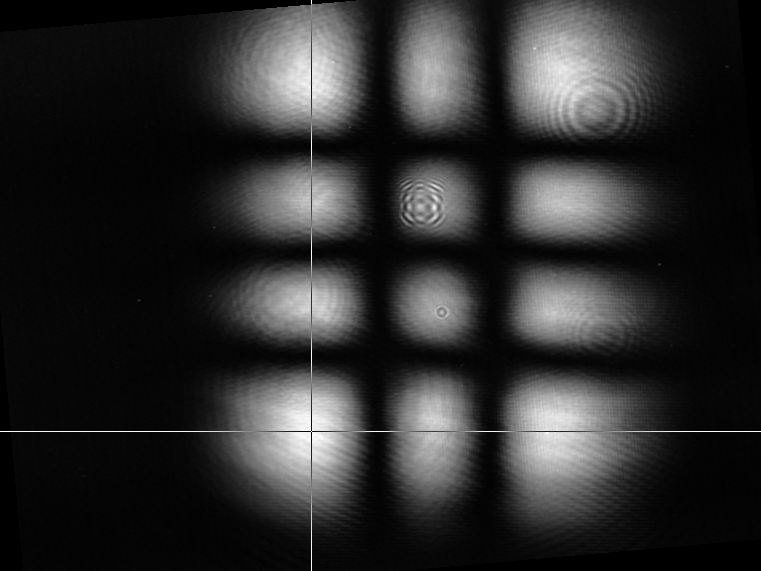
\includegraphics[width=\textwidth]{img/TEM23.png}
        \end{subfigure}%
        ~ %add desired spacing between images, e. g. ~, \quad, \qquad etc.
          %(or a blank line to force the subfigure onto a new line)
        \begin{subfigure}{0.5\textwidth}
                \begin{tikzpicture}
								\begin{axis}[
										%title={Strahlbreiten in Abhängigkeit der Resonatorlänge},
										xlabel=Pixel,
										ylabel=Intensität,
										width=0.9\textwidth,
										height=7cm,
										xmin=1,
										xmax=750,
										grid=both,
										ymin=0,
										ymax=7000,
										tick align=outside,
										tickpos=left,
										minor x tick num=3,
										minor y tick num=4,
										minor grid style={dotted,thin},
										legend pos=north east,
										yticklabels={,,},
										ylabel near ticks,
								]
								\addplot [smooth, red, thick,] table {latexdata/TEM23x.dat};
								\addlegendentry{$I_x$}

								\addplot[smooth, blue, thick] table {latexdata/TEM23y.dat};
								\addlegendentry{$I_y$}

								\end{axis}
								\end{tikzpicture}
        \end{subfigure}
	\captionof{figure}{
		TEM23-Mode, Bild gedreht um 5 Grad
	}
\end{figure}

\begin{figure}[h]
        \centering
        \begin{subfigure}{0.5\textwidth}
                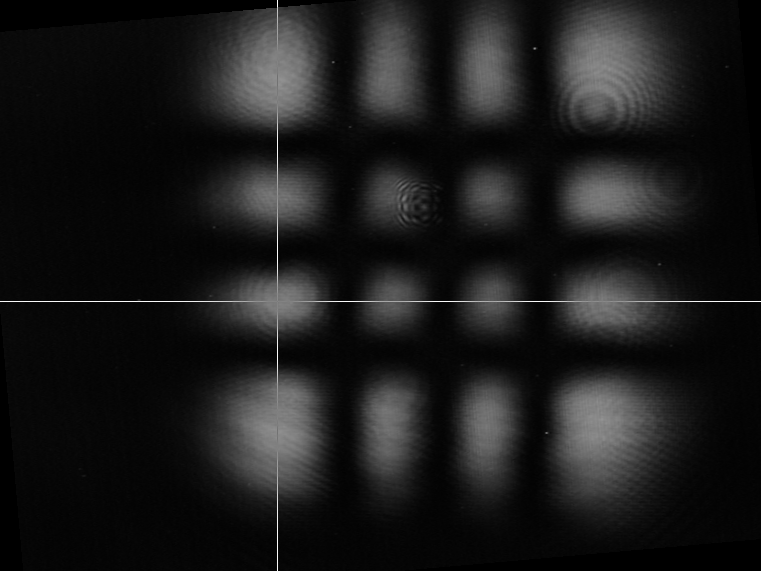
\includegraphics[width=\textwidth]{img/TEM33.png}
        \end{subfigure}%
        ~ %add desired spacing between images, e. g. ~, \quad, \qquad etc.
          %(or a blank line to force the subfigure onto a new line)
        \begin{subfigure}{0.5\textwidth}
                \begin{tikzpicture}
								\begin{axis}[
										%title={Strahlbreiten in Abhängigkeit der Resonatorlänge},
										xlabel=Pixel,
										ylabel=Intensität,
										width=0.9\textwidth,
										height=7cm,
										xmin=1,
										xmax=750,
										grid=both,
										ymin=0,
										ymax=3500,
										tick align=outside,
										tickpos=left,
										minor x tick num=3,
										minor y tick num=4,
										minor grid style={dotted,thin},
										legend pos=north east,
										yticklabels={,,},
										ylabel near ticks,
								]
								\addplot [smooth, red, thick,] table {latexdata/TEM33x.dat};
								\addlegendentry{$I_x$}

								\addplot[smooth, blue, thick] table {latexdata/TEM33y.dat};
								\addlegendentry{$I_y$}

								\end{axis}
								\end{tikzpicture}
        \end{subfigure}
	\captionof{figure}{
		TEM33-Mode, Bild gedreht um 5 Grad
	}
\end{figure}

\begin{figure}[h]
        \centering
        \begin{subfigure}{0.5\textwidth}
                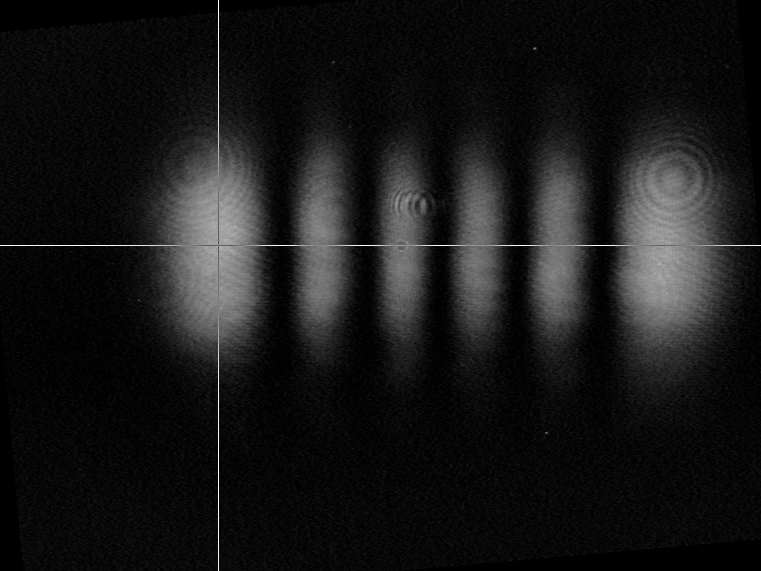
\includegraphics[width=\textwidth]{img/TEM50.png}
        \end{subfigure}%
        ~ %add desired spacing between images, e. g. ~, \quad, \qquad etc.
          %(or a blank line to force the subfigure onto a new line)
        \begin{subfigure}{0.5\textwidth}
                \begin{tikzpicture}
								\begin{axis}[
										%title={Strahlbreiten in Abhängigkeit der Resonatorlänge},
										xlabel=Pixel,
										ylabel=Intensität,
										width=0.9\textwidth,
										height=7cm,
										xmin=1,
										xmax=750,
										grid=both,
										ymin=0,
										ymax=4500,
										tick align=outside,
										tickpos=left,
										minor x tick num=3,
										minor y tick num=4,
										minor grid style={dotted,thin},
										legend pos=north east,
										yticklabels={,,},
										ylabel near ticks,
								]
								\addplot [smooth, red, thick,] table {latexdata/TEM50x.dat};
								\addlegendentry{$I_x$}

								\addplot[smooth, blue, thick] table {latexdata/TEM50y.dat};
								\addlegendentry{$I_y$}

								\end{axis}
								\end{tikzpicture}
        \end{subfigure}
	\captionof{figure}{
		TEM50-Mode, Bild gedreht um 5 Grad
	}
\end{figure}

\begin{figure}[h]
        \centering
        \begin{subfigure}{0.5\textwidth}
                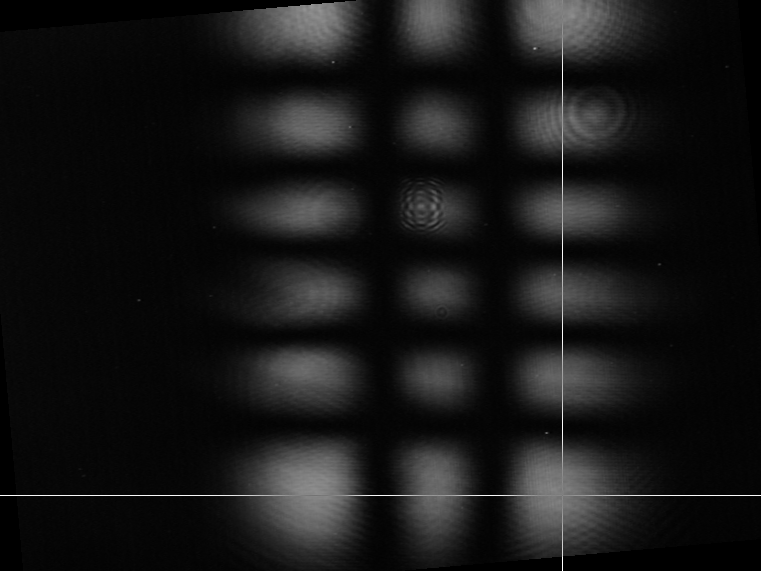
\includegraphics[width=\textwidth]{img/TEM52.png}
        \end{subfigure}%
        ~ %add desired spacing between images, e. g. ~, \quad, \qquad etc.
          %(or a blank line to force the subfigure onto a new line)
        \begin{subfigure}{0.5\textwidth}
                \begin{tikzpicture}
								\begin{axis}[
										%title={Strahlbreiten in Abhängigkeit der Resonatorlänge},
										xlabel=Pixel,
										ylabel=Intensität,
										width=0.9\textwidth,
										height=7cm,
										xmin=1,
										xmax=750,
										grid=both,
										ymin=0,
										ymax=3000,
										tick align=outside,
										tickpos=left,
										minor x tick num=3,
										minor y tick num=4,
										minor grid style={dotted,thin},
										legend pos=north east,
										yticklabels={,,},
										ylabel near ticks,
								]
								\addplot [smooth, red, thick,] table {latexdata/TEM52x.dat};
								\addlegendentry{$I_x$}

								\addplot[smooth, blue, thick] table {latexdata/TEM52y.dat};
								\addlegendentry{$I_y$}

								\end{axis}
								\end{tikzpicture}
        \end{subfigure}
	\captionof{figure}{
		TEM52-Mode, Bild gedreht um 5 Grad
	}
\end{figure}

\chapter{Auswertung}
\section{Ausgangsleistung des Lasers in Abh. von der Resonatorlänge}

\newpage
\section{Strahlbreite der Grundmode in Abh. von der Resonatorlänge}
Die Strahlbreite wird aus den gemessenen Daten gewonnen, indem auf die gemessenen Punkte ein Gauß-fit gelegt wird. Die Strahlbreite wird dann über die Formel
$w=2*\sqrt{4}\cdot\sigma$
bestimmt. Dies führt zu folgenden experimentellen und erwarteten Werten für die Strahlbreite in Abhängigkeit der Resonatorlänge:
\begin{center}
    \begin{tabular}{ | l | l | l | l | p{4cm} |}
    \hline
    $L$ in cm & $w_x\left(\frac{L}{2}\right)$ in mm & $w_y\left(\frac{L}{2}\right)$ in mm & Differenz x und y in \% & $w_{lit}$ in mm \\ \hline
    25 & 0,4924 & 0,4798 & 2,55 & 0,4742 \\ \hline
    32 & 0,7677 & 0,7491 & 2,42 & 0,5190 \\ \hline
    39 & 0,6776 & 0,6703 & 1,08 & 0,5632 \\ \hline
    46 & 0,5173 & 0,5728 & 9,69 & 0,6089 \\ \hline
    53 & 0,6358 & 0,6383 & 0,39 & 0,6588 \\ \hline
    60 & 0,6777 & 0,6899 & 1,77 & 0,7161 \\ \hline
    67 & 0,7957 & 0,7758 & 2,50 & 0,7868 \\ \hline
    74 & 0,8592 & 0,8857 & 2,99 & 0,8832 \\ \hline
    81 & 0,9856 & 1,0212 & 3,49 & 1,0431 \\ \hline
    88 & 1,4031 & 1,5161 & 7,45 & 1,5411 \\ \hline
    \end{tabular}
\end{center}

\begin{center}
\begin{figure}[h]
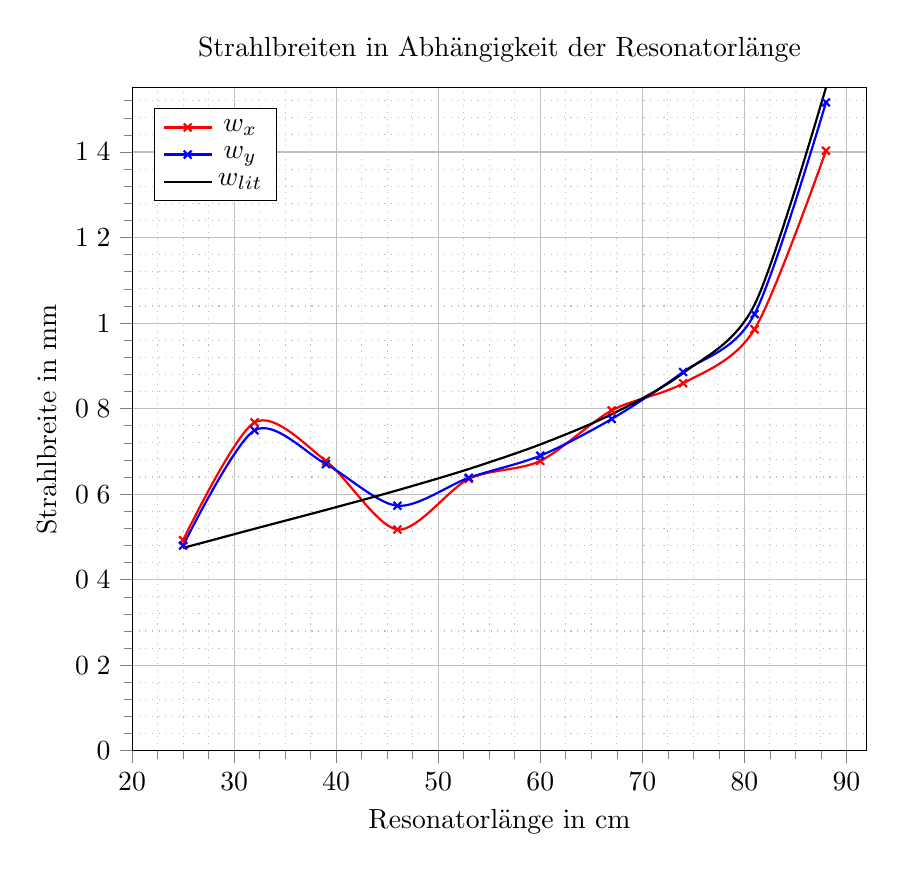
\begin{tikzpicture}
\begin{axis}[
    title={Strahlbreiten in Abhängigkeit der Resonatorlänge},
    xlabel=Resonatorlänge in cm,
    ylabel=Strahlbreite in mm,
    width=0.9\textwidth,
    height=10cm,
    xmin=20,
    xmax=92,
    grid=both,
    ymin=0,
    ymax=1.55,
    tick align=outside,
    tickpos=left,
    minor x tick num=3,
    minor y tick num=4,
    minor grid style={dotted,thin},
    legend pos=north west
]
\addplot[smooth, red, thick, mark=x, mark size=2pt] coordinates {
  (25, 0.4924) (32, 0.7677) (39, 0.6776) (46, 0.5173)
  (53, 0.6358) (60, 0.6777) (67, 0.7957) (74, 0.8592)
  (81, 0.9856) (88, 1.4031)
};
\addlegendentry{$w_x$}

\addplot[smooth, blue, thick, mark=x, mark size=2pt] coordinates {
  (25, 0.4798) (32, 0.7491) (39, 0.6703) (46, 0.5728)
  (53, 0.6383) (60, 0.6899) (67, 0.7758) (74, 0.8857)
  (81, 1.0212) (88, 1.5161)
};
\addlegendentry{$w_y$}
% \addplot[smooth, black, thick, mark size=0.0pt] coordinates{
%   (25, 0.2371) (32, 0.2595) (39, 0.2816) (46, 0.3045)
%   (53, 0.3294) (60, 0.3581) (67, 0.3934) (74, 0.4416)
%   (81, 0.5215) (88, 0.7755)
% };
\addplot[smooth, black, thick, mark size=0.0pt] coordinates{
  (25, 0.4742) (32, 0.2595*2) (39, 0.2816*2) (46, 0.3045*2)
  (53, 0.3294*2) (60, 0.3581*2) (67, 0.3934*2) (74, 0.4416*2)
  (81, 0.5215*2) (88, 0.7755*2)
};
\addlegendentry{$w_{lit}$}
\end{axis}
\end{tikzpicture}
\captionof{figure}{
  Strahlbreite als horizontaler und vertikaler Schnitt in Abhängigkeit von der Resonatorlänge.
  Die Werte für $w_x$ und $w_y$ liegen sehr gut beieinander, was auf eine relativ gute Genauigkeit der gemessenen Daten schließen lässt.
  Bis auf die Werte für 32cm und 39cm folgt der Strahlverlauf sehr gut dem theoretischen Wert.
}
\end{figure}
\end{center}
\FloatBarrier
  
\section{Longitudinale Modensruktur in Abh. von der Resonatorlänge}
Für Jede Resonatorlänge sind auf die Messdaten des Interferometers zwei Lorenzkurven gefittet. Der Abstand der Peaks dieser Kurven ist der longitudinaler Modenabstand für die jeweilige Resonatorlänge. Da das ans Interferometer angeschlossene Digitaloszilliskop den Abstand in Sekunden angibt, war zuvor die Bestimmung eines Umrechnungsfaktors von Sekunden zu GHz notwendig. Es gilt
$$8,0248s \equalhat 10GHz$$

\begin{figure}[h!]
  \centering
    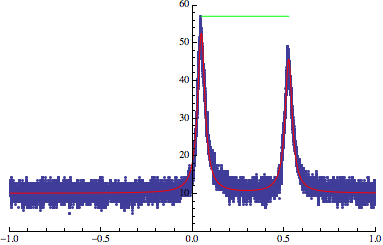
\includegraphics[width=65mm]{img/Modenabstand25cm.png}
  \caption{Zwei Lorenzkurven gefittet auf die Messpunkte aus dem Interferometer, hier am Beispiel für eine Resonatorlänge von 25cm. Die Grüne linie markiert den gemessenen Abstand zwischen den Peaks der in rot gezeichneten Fits der Lorenzkurven auf die blauen Messpunkte auf die blauen Messpunkte}
\end{figure}
\FloatBarrier

\begin{center}
  \begin{tabular}{ | p{2.3cm} | p{2.7cm} | p{2cm} | p{2.8cm} | p{5.7cm} | }
    \hline
    % Resonatorlänge & Modenabstand in ms	& Abstand in GHz & Theoretischer Abstand in GHz & stuff \\ \hline
    Resonatorlänge in cm & Modenabstand in ms & Abstand in GHz & Theoretischer Abstand in GHz & Abweichung Gemessener Abstand vom Theoriewert in \% \\ \hline
    25 & 0,4774 & 0,594937 & 0,600000 & 0,85 \\ \hline
    32 & 0,3821 & 0,476173 & 0,468750 & 1,56 \\ \hline
    39 & 0,3094 & 0,385541 & 0,384615 & 0,24 \\ \hline
    46 & 0,2609 & 0,325107 & 0,326087 & 0,30 \\ \hline
    53 & 0,2242 & 0,281910 & 0,283018 & 0,39 \\ \hline
    60 & 0,2007 & 0,250071 & 0,250000 & 0,03 \\ \hline
    67 & 0,1804 & 0,224864 & 0,223881 & 0,44 \\ \hline
    74 & 0,1635 & 0,203695 & 0,202703 & 0,49 \\ \hline
    81 & 0,1452 & 0,180879 & 0,185185 & 2,38 \\ \hline
    88 & 0,1375 & 0,171313 & 0,170454 & 0,50 \\ \hline
  \end{tabular}
\end{center}
\FloatBarrier
\begin{center}
\begin{figure}[h]
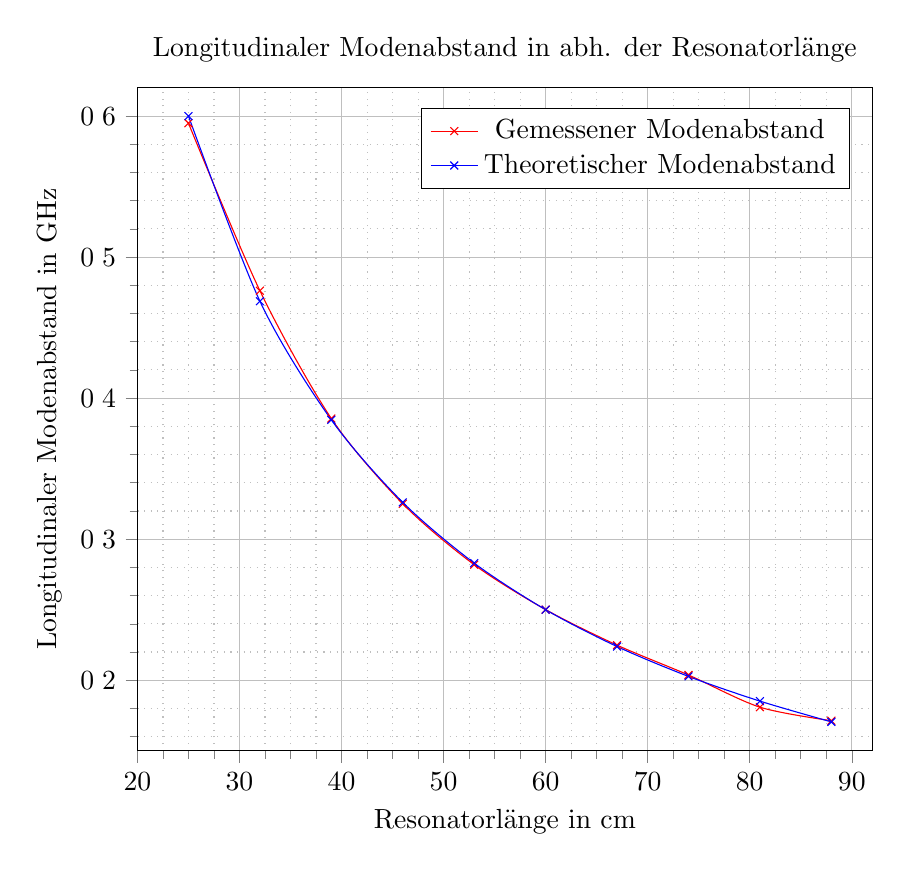
\begin{tikzpicture}
\begin{axis}[
    title={Longitudinaler Modenabstand in abh. der Resonatorlänge},
    xlabel=Resonatorlänge in cm,
    ylabel=Longitudinaler Modenabstand in GHz,
    width=0.9\textwidth,
    height=10cm,
    xmin=20,
    xmax=92,
    grid=both,
    ymin=0.15,
    ymax=0.62,
    tick align=outside,
    tickpos=left,
    minor x tick num=3,
    minor y tick num=4,
    minor grid style={dotted,thin},
    legend pos=north east
]
\addplot[smooth, red, mark=x, mark size=2pt] coordinates {
  (25, 0.594937) (32, 0.476173) (39, 0.385541) (46, 0.325107)
  (53, 0.281910) (60, 0.250071) (67, 0.224864) (74, 0.203695)
  (81, 0.180879) (88, 0.171313)
};
\addlegendentry{Gemessener Modenabstand}

\addplot[smooth, blue, mark=x, mark size=2pt] coordinates {
  (25, 0.600000) (32, 0.468750) (39, 0.384615) (46, 0.326087)
  (53, 0.283018) (60, 0.250000) (67, 0.223881) (74, 0.202703)
  (81, 0.185185) (88, 0.170454)
};
\addlegendentry{Theoretischer Modenabstand}
\end{axis}
\end{tikzpicture}
\captionof{figure}{
  Longitudinaler Modenabstand in Abhängigkeit der Resonatorlänger. Die gute Übereinstimmung der gemessenen Daten mit dem Modell $\Delta\nu = \frac{c}{2L}$ ist hier sehr schön zu sehen. Es gibt nur wenige Messpunkte, die überhaupt optisch von den theoretischen Daten zu unterscheiden sind.
}
\end{figure}
\end{center}
\FloatBarrier
Der longitudinaler Modenabstand passt praktisch perfekt auf das Modell $\Delta\nu = \frac{c}{2L}$, die größte Abweichung beträgt weniger als 2.5\% vom errechneten Wert.
\section{Verstärkungsbandbreite des HeNe-Lasers}
Die Verstärkungsbandbreite des HeNe-Lasers wird hauptsächlich durch Doppler-Verbreiterung im Lasserrohr hervorgerufen, die Verstärkungsbandbreite sollte also in etwa gaußförmiges Profil haben. Bei Verringerung der Intensität des Lasers sollte die Verstärkungsbandbreite zudem reduziert werden, da weiter außer liegende Moden unter die durch Verluste im Resonator verursachte Laserschwelle fallen.

Die Laserschwelle kommt daher zustande, dass ein Laser pro Durchlauf zwar prinzipiell alle Moden verstärkt, verluste durch Verunreinigungen am Spiegel oder auf den Fenstern des Laser-Rohres, nicht perfekte Reflektivität der Spiegel und Streuung in der Luft führen allerdings zu einem fixen Intensitätsverlust bei jedem Umlauf im Resonator. Aufgrund dessen können nur Moden, die eine höhere Verstärkung als Verluste erfahren, im Laserresonator anlaufen.

\begin{figure}[h!]
  \centering
    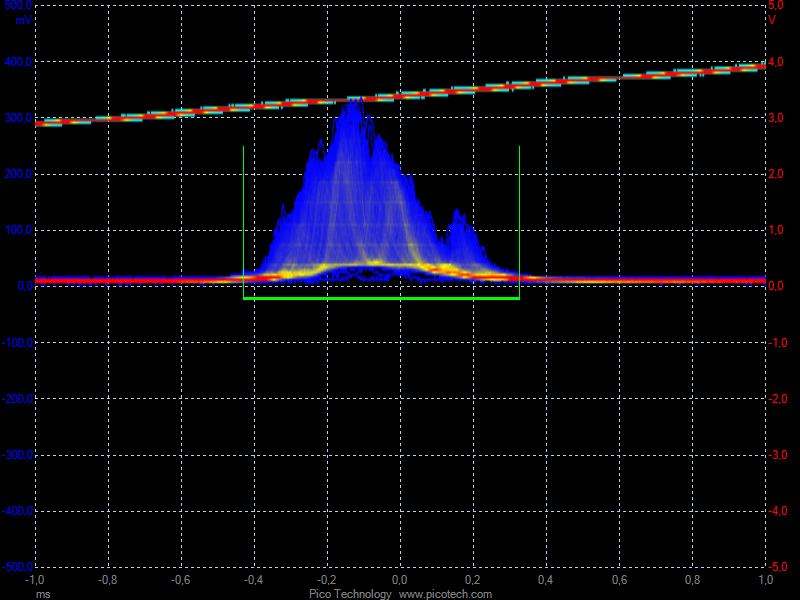
\includegraphics[width=95mm]{img/Bandbreite81cm191mW4uW.png}
  \caption{Verstärkungsprofil des HeNe-Lasers bei einer Ausgangsleistung von 191mW. Der grüne Kasten representiert die angenommene Verstärkungsbandbreite}
\end{figure}
\begin{figure}[h!]
  \centering
    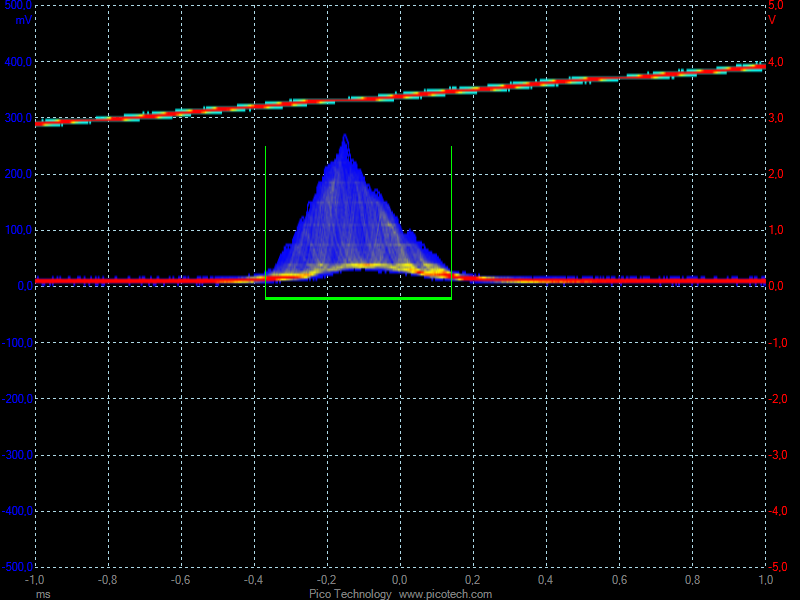
\includegraphics[width=95mm]{img/Bandbreite81cm101mW4uW.png}
  \caption{Verstärkungsprofil des HeNe-Lasers bei einer Ausgangsleistung von 101mW. Der grüne Kasten representiert die angenommene Verstärkungsbandbreite}
\end{figure}
\FloatBarrier

Mit dem aus 4.3 gewonnenen Umrechnungsfaktor $8,0248s \equalhat 10GHz$ kommen wir auf folgende Werte für die Verstärkungsbandbreite
\begin{center}
  \begin{tabular}{ | p{2.8cm} | p{3.7cm} | p{3.6cm} | p{5cm} | }
    \hline
    % Resonatorlänge & Modenabstand in ms	& Abstand in GHz & Theoretischer Abstand in GHz & stuff \\ \hline
    Resonatorlänge in cm & Ausgangsleistung in mW & Fehler der Ausgangsleistung in $\mu W$ & Verstärkungsbandbreite in GHz \\ \hline
    88 & 191 & 4 & 0,9444 \\ \hline
    88 & 101 & 4 & 0,6376 \\ \hline
  \end{tabular}
\end{center}
Da diese Werte nur graphisch bestimmt wurden mit einer Abschätzung, wo die jeweiligen Gauskurven enden, sind die gewonnenen Verstärkungsbandbreiten nur eine grobe Abschätzung der tatsächlichen Werte.

Unter der Annahme, dass die Verstärkungsbandbreite primär durch gaußförmige Dopplerverbreiterung hervorgerufen wird, sollte sich unter Vernachlässigung von Verlusten im Resonator ein gaußförmiges Verstärkungsprofil mit der Standardabweichung $\sigma = \frac{f_0}{c}\sqrt{\frac{k_b T}{m}}$ mit dem Mittelwert des Verstärlkungsprofils $f_0$, der Teilchentemperatur $T$ und der Teilchemnasse $T=20u$ ergeben. Für die Berechnung eines theoretischen Wertes für die Verstärkungsbandbreite fehlen uns leider Werte wie die mittlere Teilchentemperatur um Verstärkerrohr sowie Auskünte über Verluste im Resonator.

\section{Beobachtung höherer transversaler Moden}

Die eindimensionale Intensitätsverteilung der höheren TEM-Moden folgt (wie bereits oben erwähnt) folgendem Verlauf:

$$I_{n}(x) \propto H_n \left( \frac{x-\mu}{\sigma} \right)^2 \exp \left( \frac{-(x-\mu)^2}{\sigma^2} \right)  $$

Zur Auswertung wird versucht, durch Anpassung der Parameter \(\sigma\) und \(\mu\) (\(\mu\) erzeugt eine horizontale Verschiebung der Verteilung) einen möglichst genauen Fit der erwarteten Intensitätsverteilung über die Messdaten zu legen. Die Amplituden der Fits werden jeweils entsprechend angepasst, sodass sie in etwa zu denen der Messdaten passen.

\begin{figure}[h]
        \centering
        \begin{subfigure}{0.5\textwidth}
                \begin{tikzpicture}
								\begin{axis}[
								    title={x-Schnitt},
										xlabel=Pixel,
										ylabel=Intensität,
										width=0.9\textwidth,
										height=7cm,
										xmin=1,
										xmax=750,
										grid=both,
										ymin=0,
										ymax=7000,
										tick align=outside,
										tickpos=left,
										minor x tick num=3,
										minor y tick num=4,
										minor grid style={dotted,thin},
										legend pos=north west,
										yticklabels={,,},
										ylabel near ticks,
								]
								\addplot [smooth, blue, thick] table {latexdata/TEM23x.dat};
								\addlegendentry{$I_x$}
								
								\addplot [smooth, red, thick, domain=0:800, samples=100] {exp(-(x-421.674)^2/(77.7091^2))*1162.62*(-2+(4*(x-421.674)^2)/(77.7091^2))^2};
								\addlegendentry{$Fit$}

								\end{axis}
								\end{tikzpicture}
								\caption{
								\(\mu = 421,674\), \(\sigma = 77,7091\)
								}
        \end{subfigure}%
        ~ %add desired spacing between images, e. g. ~, \quad, \qquad etc.
          %(or a blank line to force the subfigure onto a new line)
        \begin{subfigure}{0.5\textwidth}
                \begin{tikzpicture}
								\begin{axis}[
										title={y-Schnitt},
										xlabel=Pixel,
										ylabel=Intensität,
										width=0.9\textwidth,
										height=7cm,
										xmin=1,
										xmax=750,
										grid=both,
										ymin=0,
										ymax=7000,
										tick align=outside,
										tickpos=left,
										minor x tick num=3,
										minor y tick num=4,
										minor grid style={dotted,thin},
										legend pos=north east,
										yticklabels={,,},
										ylabel near ticks,
								]

								\addplot[smooth, blue, thick] table {latexdata/TEM23y.dat};
								\addlegendentry{$I_y$}
								
								\addplot [smooth, red, thick, domain=0:800, samples=100] {exp(-(x-248.956)^2/(85.9621^2))*224.818*((8*(x-248.956)^3)/(85.9621^3) -(12*(x-248.956))/(85.9621))^2};
								\addlegendentry{$Fit$}

								\end{axis}
								\end{tikzpicture}
								\caption{
								\(\mu = 248,956\), \(\sigma = 85,9621\)
								}
        \end{subfigure}
	\captionof{figure}{
		TEM23-Mode: Vergleich der gemessenen mit der erwarteten Intensitätsverteilung
	}
\end{figure}

\begin{figure}[h]
        \centering
        \begin{subfigure}{0.5\textwidth}
                \begin{tikzpicture}
								\begin{axis}[
								    title={x-Schnitt},
										xlabel=Pixel,
										ylabel=Intensität,
										width=0.9\textwidth,
										height=7cm,
										xmin=1,
										xmax=750,
										grid=both,
										ymin=0,
										ymax=3000,
										tick align=outside,
										tickpos=left,
										minor x tick num=3,
										minor y tick num=4,
										minor grid style={dotted,thin},
										legend pos=north west,
										yticklabels={,,},
										ylabel near ticks,
								]
								\addplot [smooth, blue, thick] table {latexdata/TEM33x.dat};
								\addlegendentry{$I_x$}
								
								\addplot [smooth, red, thick, domain=0:800, samples=100] {exp(-(x-442.4)^2/(78.7475^2))*68.7467*((8*(x-442.4)^3)/(78.7475^3) -(12*(x-442.4))/(78.7475))^2};
								\addlegendentry{$Fit$}

								\end{axis}
								\end{tikzpicture}
								\caption{
								\(\mu = 442,400\), \(\sigma = 78,7475\)
								}
        \end{subfigure}%
        ~ %add desired spacing between images, e. g. ~, \quad, \qquad etc.
          %(or a blank line to force the subfigure onto a new line)
        \begin{subfigure}{0.5\textwidth}
                \begin{tikzpicture}
								\begin{axis}[
										title={y-Schnitt},
										xlabel=Pixel,
										ylabel=Intensität,
										width=0.9\textwidth,
										height=7cm,
										xmin=1,
										xmax=750,
										grid=both,
										ymin=0,
										ymax=3000,
										tick align=outside,
										tickpos=left,
										minor x tick num=3,
										minor y tick num=4,
										minor grid style={dotted,thin},
										legend pos=north east,
										yticklabels={,,},
										ylabel near ticks,
								]

								\addplot[smooth, blue, thick] table {latexdata/TEM33y.dat};
								\addlegendentry{$I_y$}
								
								\addplot [smooth, red, thick, domain=0:800, samples=100] {exp(-(x-244.328)^2/(84.807^2))*91.7463*((8*(x-244.328)^3)/(84.807^3) -(12*(x-244.328))/(84.807))^2};
								\addlegendentry{$Fit$}

								\end{axis}
								\end{tikzpicture}
								\caption{
								\(\mu = 244,328\), \(\sigma = 84,807\)
								}
        \end{subfigure}
	\captionof{figure}{
		TEM33-Mode: Vergleich der gemessenen mit der erwarteten Intensitätsverteilung
	}
\end{figure}

\begin{figure}[h]
        \centering
        \begin{subfigure}{0.5\textwidth}
                \begin{tikzpicture}
								\begin{axis}[
								    title={x-Schnitt},
										xlabel=Pixel,
										ylabel=Intensität,
										width=0.9\textwidth,
										height=7cm,
										xmin=1,
										xmax=750,
										grid=both,
										ymin=0,
										ymax=4000,
										tick align=outside,
										tickpos=left,
										minor x tick num=3,
										minor y tick num=4,
										minor grid style={dotted,thin},
										legend pos=north west,
										yticklabels={,,},
										ylabel near ticks,
								]
								\addplot [smooth, blue, thick] table {latexdata/TEM50x.dat};
								\addlegendentry{$I_x$}
								
								\addplot [smooth, red, thick, domain=0:800, samples=100] {exp(-(x-440.895)^2/(80.112^2))*1.4719*((32*(x-440.895)^5)/(80.112^5) - (160*(x-440.895)^3)/(80.112^3) +(120*(x-440.895))/(80.112))^2};
								\addlegendentry{$Fit$}

								\end{axis}
								\end{tikzpicture}
								\caption{
								\(\mu = 440,895\), \(\sigma = 80,112\)
								}
        \end{subfigure}%
        ~ %add desired spacing between images, e. g. ~, \quad, \qquad etc.
          %(or a blank line to force the subfigure onto a new line)
        \begin{subfigure}{0.5\textwidth}
                \begin{tikzpicture}
								\begin{axis}[
										title={y-Schnitt},
										xlabel=Pixel,
										ylabel=Intensität,
										width=0.9\textwidth,
										height=7cm,
										xmin=1,
										xmax=750,
										grid=both,
										ymin=0,
										ymax=4000,
										tick align=outside,
										tickpos=left,
										minor x tick num=3,
										minor y tick num=4,
										minor grid style={dotted,thin},
										legend pos=north east,
										yticklabels={,,},
										ylabel near ticks,
								]

								\addplot[smooth, blue, thick] table {latexdata/TEM50y.dat};
								\addlegendentry{$I_y$}
								
								\addplot [smooth, red, thick, domain=0:800, samples=100] {exp(-(x-231.669)^2/(84.4827^2))*3597.15};
								\addlegendentry{$Fit$}

								\end{axis}
								\end{tikzpicture}
								\caption{
								\(\mu = 231,669\), \(\sigma = 84,4827\)
								}
        \end{subfigure}
	\captionof{figure}{
		TEM50-Mode: Vergleich der gemessenen mit der erwarteten Intensitätsverteilung
	}
\end{figure}

\begin{figure}[h]
        \centering
        \begin{subfigure}{0.5\textwidth}
                \begin{tikzpicture}
								\begin{axis}[
								    title={x-Schnitt},
										xlabel=Pixel,
										ylabel=Intensität,
										width=0.9\textwidth,
										height=7cm,
										xmin=1,
										xmax=750,
										grid=both,
										ymin=0,
										ymax=3000,
										tick align=outside,
										tickpos=left,
										minor x tick num=3,
										minor y tick num=4,
										minor grid style={dotted,thin},
										legend pos=north west,
										yticklabels={,,},
										ylabel near ticks,
								]
								\addplot [smooth, blue, thick] table {latexdata/TEM52x.dat};
								\addlegendentry{$I_x$}
								
								\addplot [smooth, red, thick, domain=0:800, samples=100] {exp(-(x-419.064)^2/(75.4268^2))*444.784*(-2+(4*(x-419.064)^2)/(75.4268^2))^2};
								\addlegendentry{$Fit$}

								\end{axis}
								\end{tikzpicture}
								\caption{
								\(\mu = 419,064\), \(\sigma = 75,4268\)
								}
        \end{subfigure}%
        ~ %add desired spacing between images, e. g. ~, \quad, \qquad etc.
          %(or a blank line to force the subfigure onto a new line)
        \begin{subfigure}{0.5\textwidth}
                \begin{tikzpicture}
								\begin{axis}[
										title={y-Schnitt},
										xlabel=Pixel,
										ylabel=Intensität,
										width=0.9\textwidth,
										height=7cm,
										xmin=1,
										xmax=750,
										grid=both,
										ymin=0,
										ymax=3000,
										tick align=outside,
										tickpos=left,
										minor x tick num=3,
										minor y tick num=4,
										minor grid style={dotted,thin},
										legend pos=north east,
										yticklabels={,,},
										ylabel near ticks,
								]

								\addplot[smooth, blue, thick] table {latexdata/TEM52y.dat};
								\addlegendentry{$I_y$}
								
								\addplot [smooth, red, thick, domain=0:800, samples=100] {exp(-(x-252.043)^2/(86.0702^2))*1.02425*((32*(x-252.043)^5)/(86.0702^5) - (160*(x-252.043)^3)/(86.0702^3) +(120*(x-252.043))/(86.0702))^2};
								\addlegendentry{$Fit$}

								\end{axis}
								\end{tikzpicture}
								\caption{
								\(\mu = 252,043\), \(\sigma = 86,0702\)
								}
        \end{subfigure}
	\captionof{figure}{
		TEM52-Mode: Vergleich der gemessenen mit der erwarteten Intensitätsverteilung
	}
\end{figure}

Anhand der Graphen erkennt man deutlich, dass die gemessenen Intensitätsverteilungen immer sehr nahe bei den theoretischen Erwartungen liegen. Die geringen sichtbaren Abweichungen haben verschiedene Ursachen, so erzeugt zum Beispiel Schmutz auf dem CCD-Sensor Interferenzeffekte (deutlich sichtbare Ringe auf den Bildern der TEM-Moden) und dadurch Verfälschungen der Intensitätsverteilungen. Auch Schwankungen der Laserintensität während des Messzeitraumes von 1 Sekunde erzeugen Abweichungen. Zusammenfassend kann man aber sagen, dass alle Ungenauigkeiten vertretbar sind und die qualitativen theoretischen Erwartungen sehr gut in der Praxis bestätigt wurden.

\chapter{Fazit}


%ENDE INHALT

\cleardoublepage{}
% Eintrag fürs Inhaltsverzeichnis

\newpage

\begin{thebibliography}{100}
  \bibitem{mappe} Literaturmappe zum Versuch aus der physikalischen Bibliothek
  \bibitem{HeNeNiveaus} \verb|http://lp.uni-goettingen.de/get/image/5074|
  \bibitem{TransModeIntensity} \verb|http://en.wikipedia.org/w/index.php?title=Transverse_mode&oldid=579051975|
\end{thebibliography}

\cleardoublepage{}
% Eintrag fürs Inhaltsverzeichnis
% Abbildungsverzeichnis einfügen
\addcontentsline{toc}{chapter}{Abbildungsverzeichnis}
\listoffigures

\end{document}
